\documentclass[a4paper]{article}


\usepackage[T1]{fontenc}    
\usepackage[utf8]{inputenc} 
\usepackage{textcomp}      
\date{} 					
\author{}                   
\usepackage{geometry}		
\geometry{ left=2cm, right=2cm, top=2cm, bottom=4cm, bindingoffset=5mm}

\usepackage{listings}
\usepackage{color}
\usepackage{longtable}
\usepackage{tikz}
\usetikzlibrary{arrows,automata}

\usepackage{pgf}


\definecolor{eminence}{RGB}{108,48,130}
\definecolor{myblue}{RGB}{65,105,225}


\lstset{
	keywordstyle=\color{myblue},  
	numbers=left,  
	stringstyle=\color{mymauve},
	numberstyle=\tiny\color{mygray} ,    
	commentstyle=\fontsize{9}{13}\itshape\color{mygreen}
}

\lstset{literate=
	{á}{{\'a}}1 {é}{{\'e}}1 {í}{{\'i}}1 {ó}{{\'o}}1 {ú}{{\'u}}1
	{Á}{{\'A}}1 {É}{{\'E}}1 {Í}{{\'I}}1 {Ó}{{\'O}}1 {Ú}{{\'U}}1
	{à}{{\`a}}1 {è}{{\`e}}1 {ì}{{\`i}}1 {ò}{{\`o}}1 {ù}{{\`u}}1
	{À}{{\`A}}1 {È}{{\'E}}1 {Ì}{{\`I}}1 {Ò}{{\`O}}1 {Ù}{{\`U}}1
	{ä}{{\"a}}1 {ë}{{\"e}}1 {ï}{{\"i}}1 {ö}{{\"o}}1 {ü}{{\"u}}1
	{Ä}{{\"A}}1 {Ë}{{\"E}}1 {Ï}{{\"I}}1 {Ö}{{\"O}}1 {Ü}{{\"U}}1
	{â}{{\^a}}1 {ê}{{\^e}}1 {î}{{\^i}}1 {ô}{{\^o}}1 {û}{{\^u}}1
	{Â}{{\^A}}1 {Ê}{{\^E}}1 {Î}{{\^I}}1 {Ô}{{\^O}}1 {Û}{{\^U}}1
	{œ}{{\oe}}1 {Œ}{{\OE}}1 {æ}{{\ae}}1 {Æ}{{\AE}}1 %{ß}{{\ss}}1
	{ű}{{\H{u}}}1 {Ű}{{\H{U}}}1 {ő}{{\H{o}}}1 {Ő}{{\H{O}}}1
	{ç}{{\c c}}1 {Ç}{{\c C}}1 {ø}{{\o}}1 {å}{{\r a}}1 {Å}{{\r A}}1
}


\usepackage{graphicx}
\usepackage{xcolor}
\usepackage{hyperref} 
\usepackage{fancyhdr}
\usepackage{amsmath}
\usepackage{caption}
\usepackage{enumitem}										
\pagestyle{fancy}
\fancyhf{}
\fancyhead[R]{2973140 - Felix Bühler  \\ 2893121 - Jan Leusmann \\  3141241 - Jamie Ullerich}
\fancyhead[L]{Scientific Visualisation \\ Sommersemester 2019 }
\renewcommand{\headrulewidth}{0.5pt} 				

\title{Exercise 10}

\begin{document}

\maketitle 
\thispagestyle{fancy}


\section*{Exercise 11. 1 - Splatting}

\newpage
\section*{Exercise 11. 2 - Meshed Polyhedra Visibility Ordering (MPVO)}

\begin{figure}[!ht]
	\centering
	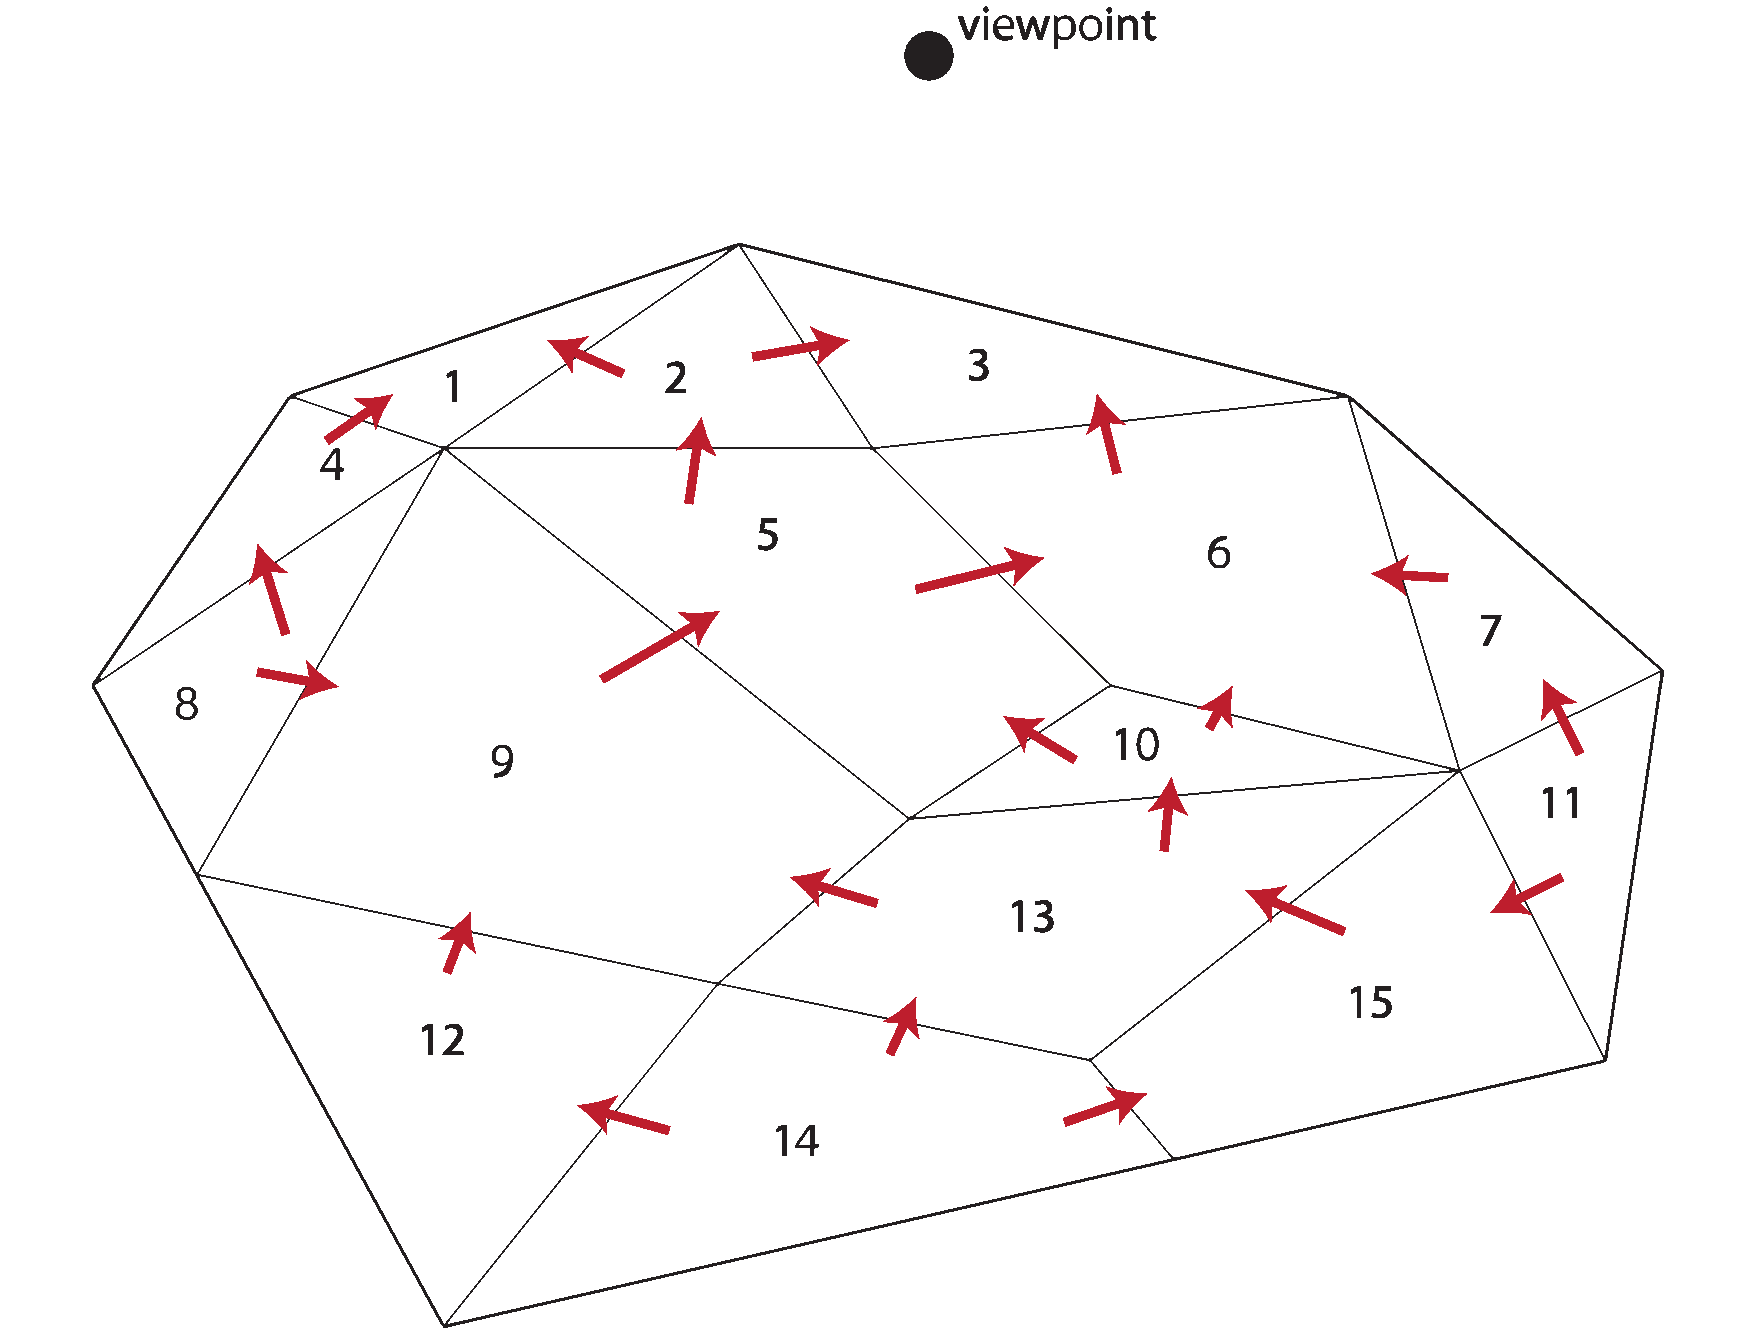
\includegraphics[width=0.7\linewidth]{neighborhoodGraph}
	\caption{neighborhoodgraph}
	\label{fig:neighborhoodgraph}
\end{figure}

\begin{figure}[!ht]
	\centering
	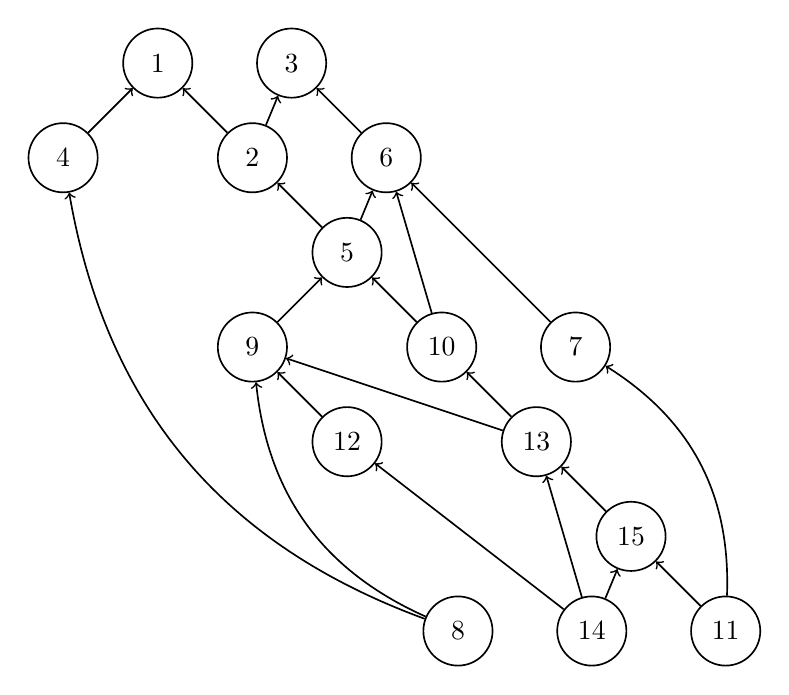
\begin{tikzpicture}[->,node distance=1.7cm,semithick]
	
	\node[state] (1) {1};
	\node[state] (3) [right of=1] {3};
	\node[state] (2) [below right of=1] {2};
	\node[state] (4) [below left of=1] {4};
	\node[state] (6) [below right of=3] {6};
	\node[state] (5) [below right of=2] {5};
	\node[state] (10) [below right of=5] {10};
	\node[state] (9) [below left of=5] {9};
	\node[state] (7) [right of=10] {7};
	\node[state] (12) [below right of=9] {12};
	\node[state] (13) [below right of=10] {13};
	\node[state] (15) [below right of=13] {15};
	\node[state] (11) [below right of=15] {11};
	\node[state] (14) [left of=11] {14};
	\node[state] (8) [left of=14] {8};
	
	\path (2) edge (1)
	          edge (3)
	      (4) edge (1)
	      (5) edge (2)
	          edge (6)
	      (6) edge (3)
	      (7) edge (6)
	      (8) edge [bend left] (4)
	          edge [bend left] (9)
	      (9) edge (5)
	      (10) edge (5)
	           edge (6)
	      (11) edge [bend right] (7)
	           edge (15)
	      (12) edge (9)
	      (13) edge (9)
	           edge (10)
	      (14) edge (12)
	           edge (13)
	           edge (15)
	      (15) edge (13);
	\end{tikzpicture}
	\caption{acyclic graph}
	\label{fig:acycligraph}
\end{figure}

\begin{itemize}
	\item Sink cells: 1, 3
	\item Source cells: 8, 11, 14
\end{itemize}

\end{document}